% main.tex or appendix.tex
\documentclass[a4paper,12pt]{article}
\usepackage{vamstyle}

\usepackage{import}
\usepackage{subfiles}

% Document
\title{Full Paper}
\author{Omar Iskandarani}
\date{\today}

\begin{document}

\begin{titlepage}
    \thispagestyle{empty}
    \centering
    \vspace*{2cm}
    {\Huge\bfseries Time Dilation in a 3D Superfluid Æther Model \par}
    \vspace{0.5cm}
    {\Large Based on Vortex Core Rotation and Ætheric Flow \par}
    \vspace{0.5cm}
    {\Large\itshape Omar Iskandarani\par}
    \vspace{0.5cm}
    \textit{Independent Researcher, Groningen, The Netherlands} \\
    ORCID: \href{https://orcid.org/0009-0006-1686-3961}{0009-0006-1686-3961} \\
    DOI: \href{https://doi.org/10.5281/zenodo.15566319}{10.5281/zenodo.15566319} \\
    {\large \today\par}


    \begin{figure}[ht]
        \centering
        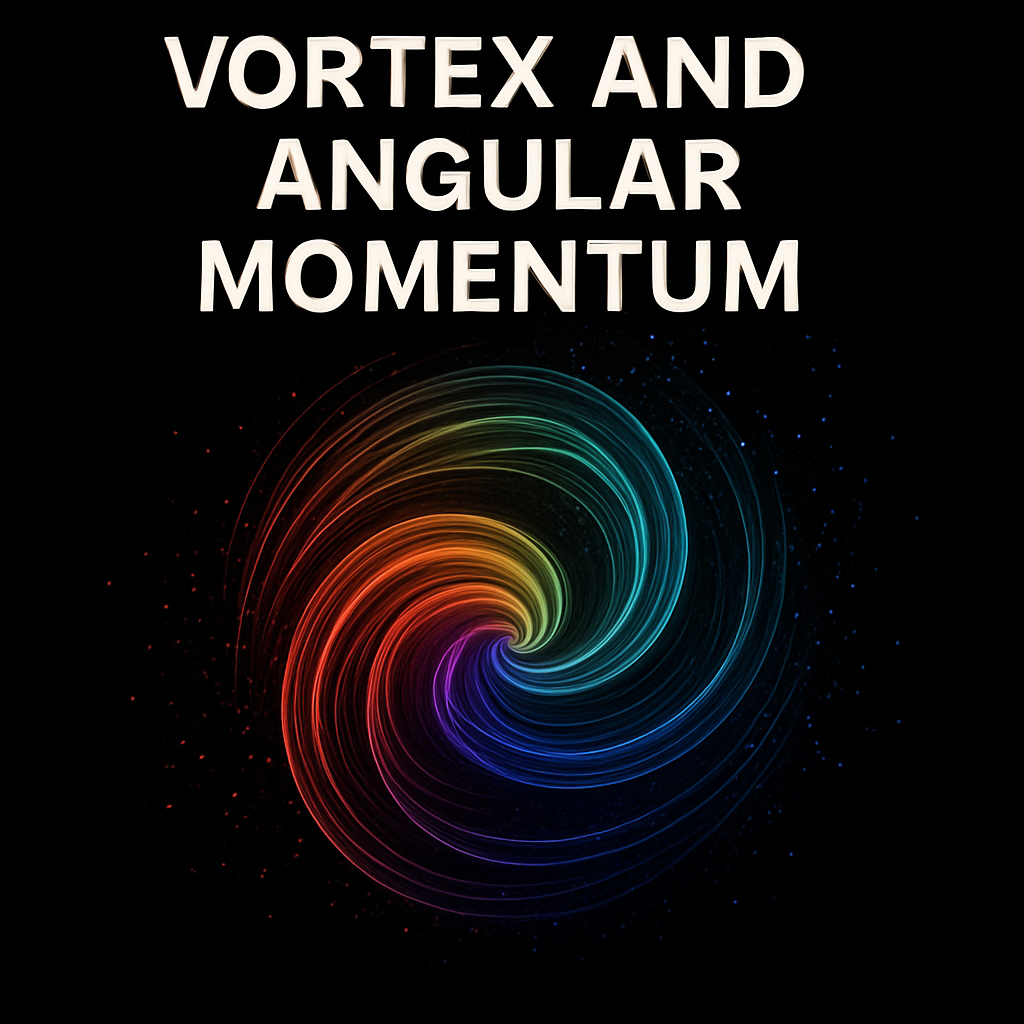
\includegraphics[width=0.85\textwidth]{images/image_vortex}
        \caption{Universal time dilation formula in the Vortex Æther Model. The clock rate decreases with increasing relative velocity~$|\vec{v}_{\mathrm{rel}}|$ with respect to the æther. At $|\vec{v}_{\mathrm{rel}}| = c$ time stops.}
        \label{fig:TijdsvertragingRelatieveBeweging}
    \end{figure}

\end{titlepage}

    \tableofcontents



    \appendix
    \def\standalonechapter{false}
    \subfile{sections/500_movement_of_free_Æther_particles.tex}  % Sets standalone=false
    \subfile{sections/510_vortex_pressure.tex}  % Sets standalone=false
    \subfile{sections/520_vorticity_natural_coords.tex}
    \subfile{sections/530_FundamentalEquationsOfVortexDynamics.tex}
    \subfile{sections/540_relative_vorticity_2knots.tex}

    \bibliographystyle{unsrt}
    \bibliography{../references}

\end{document}